\documentclass[a4paper]{article}
\usepackage[T2A]{fontenc}
\usepackage[utf8]{inputenc}
\usepackage{graphicx}
\usepackage{wrapfig}
\usepackage{enumitem}
\usepackage{caption}
\captionsetup{justification=centering}
\usepackage[english, russian]{babel}
\usepackage{amsmath}
\usepackage{geometry}
\usepackage{longtable}
\setcounter{totalnumber}{5}

\geometry{verbose, a4paper, tmargin=2cm, bmargin=2cm, lmargin=2.0cm, rmargin=2.0cm}

\begin{document}
	
	\begin{titlepage}
		\centering
		{\scshape\Large МОСКОВСКИЙ ФИЗИКО-ТЕХНИЧЕСКИЙ ИНСТИТУТ \\
			(НАЦИОНАЛЬНЫЙ ИССЛЕДОВАТЕЛЬСКИЙ УНИВЕРСИТЕТ)\\
			Физтех-школа аэрокосмических технологий}
		
		\vspace{4cm}
		{\LARGE Отчет о выполнении лабораторной работы 3.3.2}
		\vspace{1cm}
		
		{\huge\bf Исследование вольт-амперной характеристики вакуумного диода}
		
		\vspace{1cm}
		\vfill
		
		\begin{flushright}
			{\LARGE Губарев Никита, Б03-502} \\
			{\LARGE Варлевский Александр, Б03-502}
		\end{flushright}
		\vfill 
		\today
	\end{titlepage}
	
	\tableofcontents
	
	\section{Аннотация}
	Цель работы: измерение удельного заряда электрона $e/m$ на основе закона «трёх вторых» для вакуумного диода. В работе исследуются вольт-амперные характеристики диода при различных токах накала, определяется область применимости закона Чайлда–Ленгмюра и по наклону зависимостей $I_a(U_a^{3/2})$ вычисляется удельный заряд электрона.
	
	\section{Описание работы}
	
	\subsection{Теоретические сведения}
	
	В режиме объёмного заряда ток в вакуумном диоде подчиняется закону «трёх вторых» (закон Чайлда–Ленгмюра). Для плоского диода:
	\[
	I = A U^{3/2}, \qquad A = \frac{4}{9} \varepsilon_0 \frac{S}{d^2} \sqrt{\frac{2e}{m}},
	\]
	где $S$ — площадь катода, $d$ — расстояние между электродами.
	
	В данной работе используется диод с цилиндрическими электродами. Для такой геометрии закон «трёх вторых» сохраняется, но коэффициент $A$ модифицируется:
	\[
	I = \alpha \cdot \frac{4}{9} \varepsilon_0 \frac{2\pi l}{r_a} \sqrt{\frac{2e}{m}} \, U^{3/2},
	\]
	где $l$ — длина катода, $r_a$ — радиус анода, $\alpha$ — поправочный коэффициент. Для нашего диода $\alpha = 0.98$.
	
	Таким образом, построив зависимость $I(U^{3/2})$ и определив её наклон $k$ в области линейности, можно найти удельный заряд:
	\[
	\frac{e}{m} = \frac{1}{2} \left( \frac{k}{\frac{4}{9} \varepsilon_0 \frac{2\pi l}{r_a} \alpha} \right)^2,
	\]
	где $k$ выражено в А/В$^{3/2}$.
	
	\subsection{Схема эксперимента}
	
	Схема установки представлена на рис.~\ref{fig:scheme} . Исследуется диод 2Ц2С с оксидным катодом. Параметры диода:
	\begin{itemize}
		\item радиус катода $r_k = 0.9$ мм;
		\item радиус анода $r_a = 9.5$ мм;
		\item длина эмитирующей части катода $l = 9$ мм;
		\item коэффициент $\alpha = 0.98$.
	\end{itemize}
	Анодное напряжение подаётся от стабилизированного источника, ток измеряется мультиметром с автоматическим переключением пределов. Ток накала устанавливается отдельным источником и контролируется амперметром.
	
	\begin{figure}[h]
		\centering
		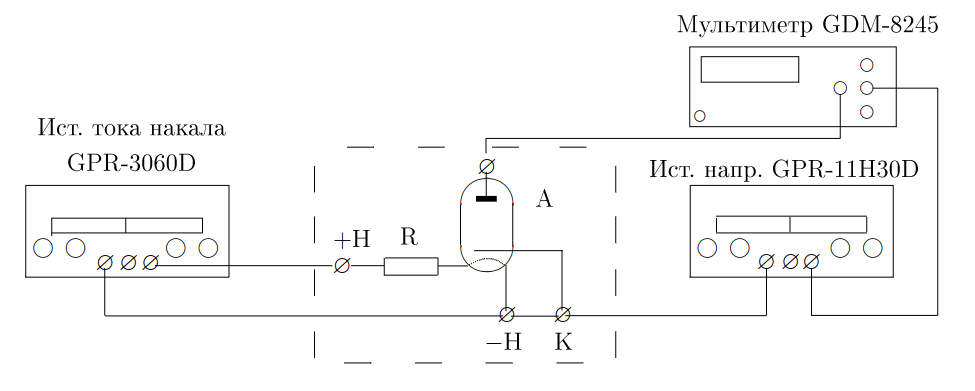
\includegraphics[width=0.6\textwidth]{scheme.png}
		\caption{Схема экспериментальной установки}
		\label{fig:scheme}
	\end{figure}
	
	\section{Методика измерений}
	
	Измерения проводились при четырёх значениях тока накала: 1.3, 1.4, 1.5 и 1.6 А. Для каждого тока накала анодное напряжение изменялось от 0.5 до 50 В. В диапазоне 0--6 В шаг составлял 0.5 В, 6--10 В — 1 В, 10--50 В — 5 В. Мультиметр работал в режиме измерения постоянного тока; для малых токов (до 10 В) использовался предел мкА, для больших — мА. Пересчёт в миллиамперы производился с учётом показаний прибора и предела измерений.
	
	Измерения начинали через 3--4 минуты после установки тока накала для стабилизации температуры катода. В процессе измерений следили за постоянством тока накала.
	
	\section{Результаты измерений}
	
	В таблице~\ref{tab:data} приведены экспериментальные значения анодного тока $I_a$ (в мА) при различных напряжениях $U_a$ (в В) для всех четырёх токов накала.
	
	\begin{longtable}{|c|c|c|c|c|}
		\hline
		$U_a$, В & $I_a$ (1.3 А), мА & $I_a$ (1.4 А), мА & $I_a$ (1.5 А), мА & $I_a$ (1.6 А), мА \\
		\hline
		0.5  & 0.00268  & 0.00429  & 0.00881  & 0.01401  \\
		1.0  & 0.00859  & 0.01340  & 0.02065  & 0.02805  \\
		1.5  & 0.02003  & 0.02567  & 0.03459  & 0.04343  \\
		2.0  & 0.03275  & 0.03946  & 0.05049  & 0.06253  \\
		2.5  & 0.04728  & 0.05835  & 0.06995  & 0.08256  \\
		3.0  & 0.06601  & 0.07448  & 0.09055  & 0.10415  \\
		3.5  & 0.08359  & 0.09405  & 0.11076  & 0.12571  \\
		4.0  & 0.10165  & 0.11471  & 0.13020  & 0.14790  \\
		4.5  & 0.12248  & 0.13846  & 0.15649  & 0.17491  \\
		5.0  & 0.14406  & 0.15865  & 0.17802  & 0.19870  \\
		5.5  & 0.16770  & 0.18158  & 0.20535  & 0.22441  \\
		6.0  & 0.19320  & 0.20881  & 0.23063  & 0.25511  \\
		7.0  & 0.24770  & 0.26705  & 0.28840  & 0.31233  \\
		8.0  & 0.30525  & 0.32878  & 0.35381  & 0.37717  \\
		9.0  & 0.36880  & 0.39137  & 0.41778  & 0.44848  \\
		10.0 & 0.42915  & 0.45875  & 0.51460  & 0.55320  \\
		15.0 & 0.83840  & 0.88720  & 0.92430  & 0.96960  \\
		20.0 & 1.32650  & 1.38520  & 1.43520  & 1.48940  \\
		25.0 & 1.88970  & 1.96570  & 2.02800  & 2.08930  \\
		30.0 & 2.50540  & 2.59650  & 2.67300  & 2.75100  \\
		35.0 & 3.17300  & 3.29520  & 3.36880  & 3.45470  \\
		40.0 & 3.88880  & 4.02690  & 4.13070  & 4.22220  \\
		45.0 & 4.63360  & 4.82680  & 4.93090  & 5.02530  \\
		50.0 & 5.48500  & 5.74600  & 5.86700  & 5.97600  \\
		\hline
		\caption{Экспериментальные данные}
		\label{tab:data}
	\end{longtable}
	
	\section{Обработка результатов}
	
	\subsection{Сырые вольт-амперные характеристики}
	
	На рис.~\ref{fig:raw} приведены экспериментальные зависимости тока от напряжения (сырые данные) с погрешностями. Видно, что все кривые имеют схожий вид: при малых напряжениях ток растёт быстрее, чем при больших, что соответствует режиму пространственного заряда.
	
	\begin{figure}[h]
		\centering
		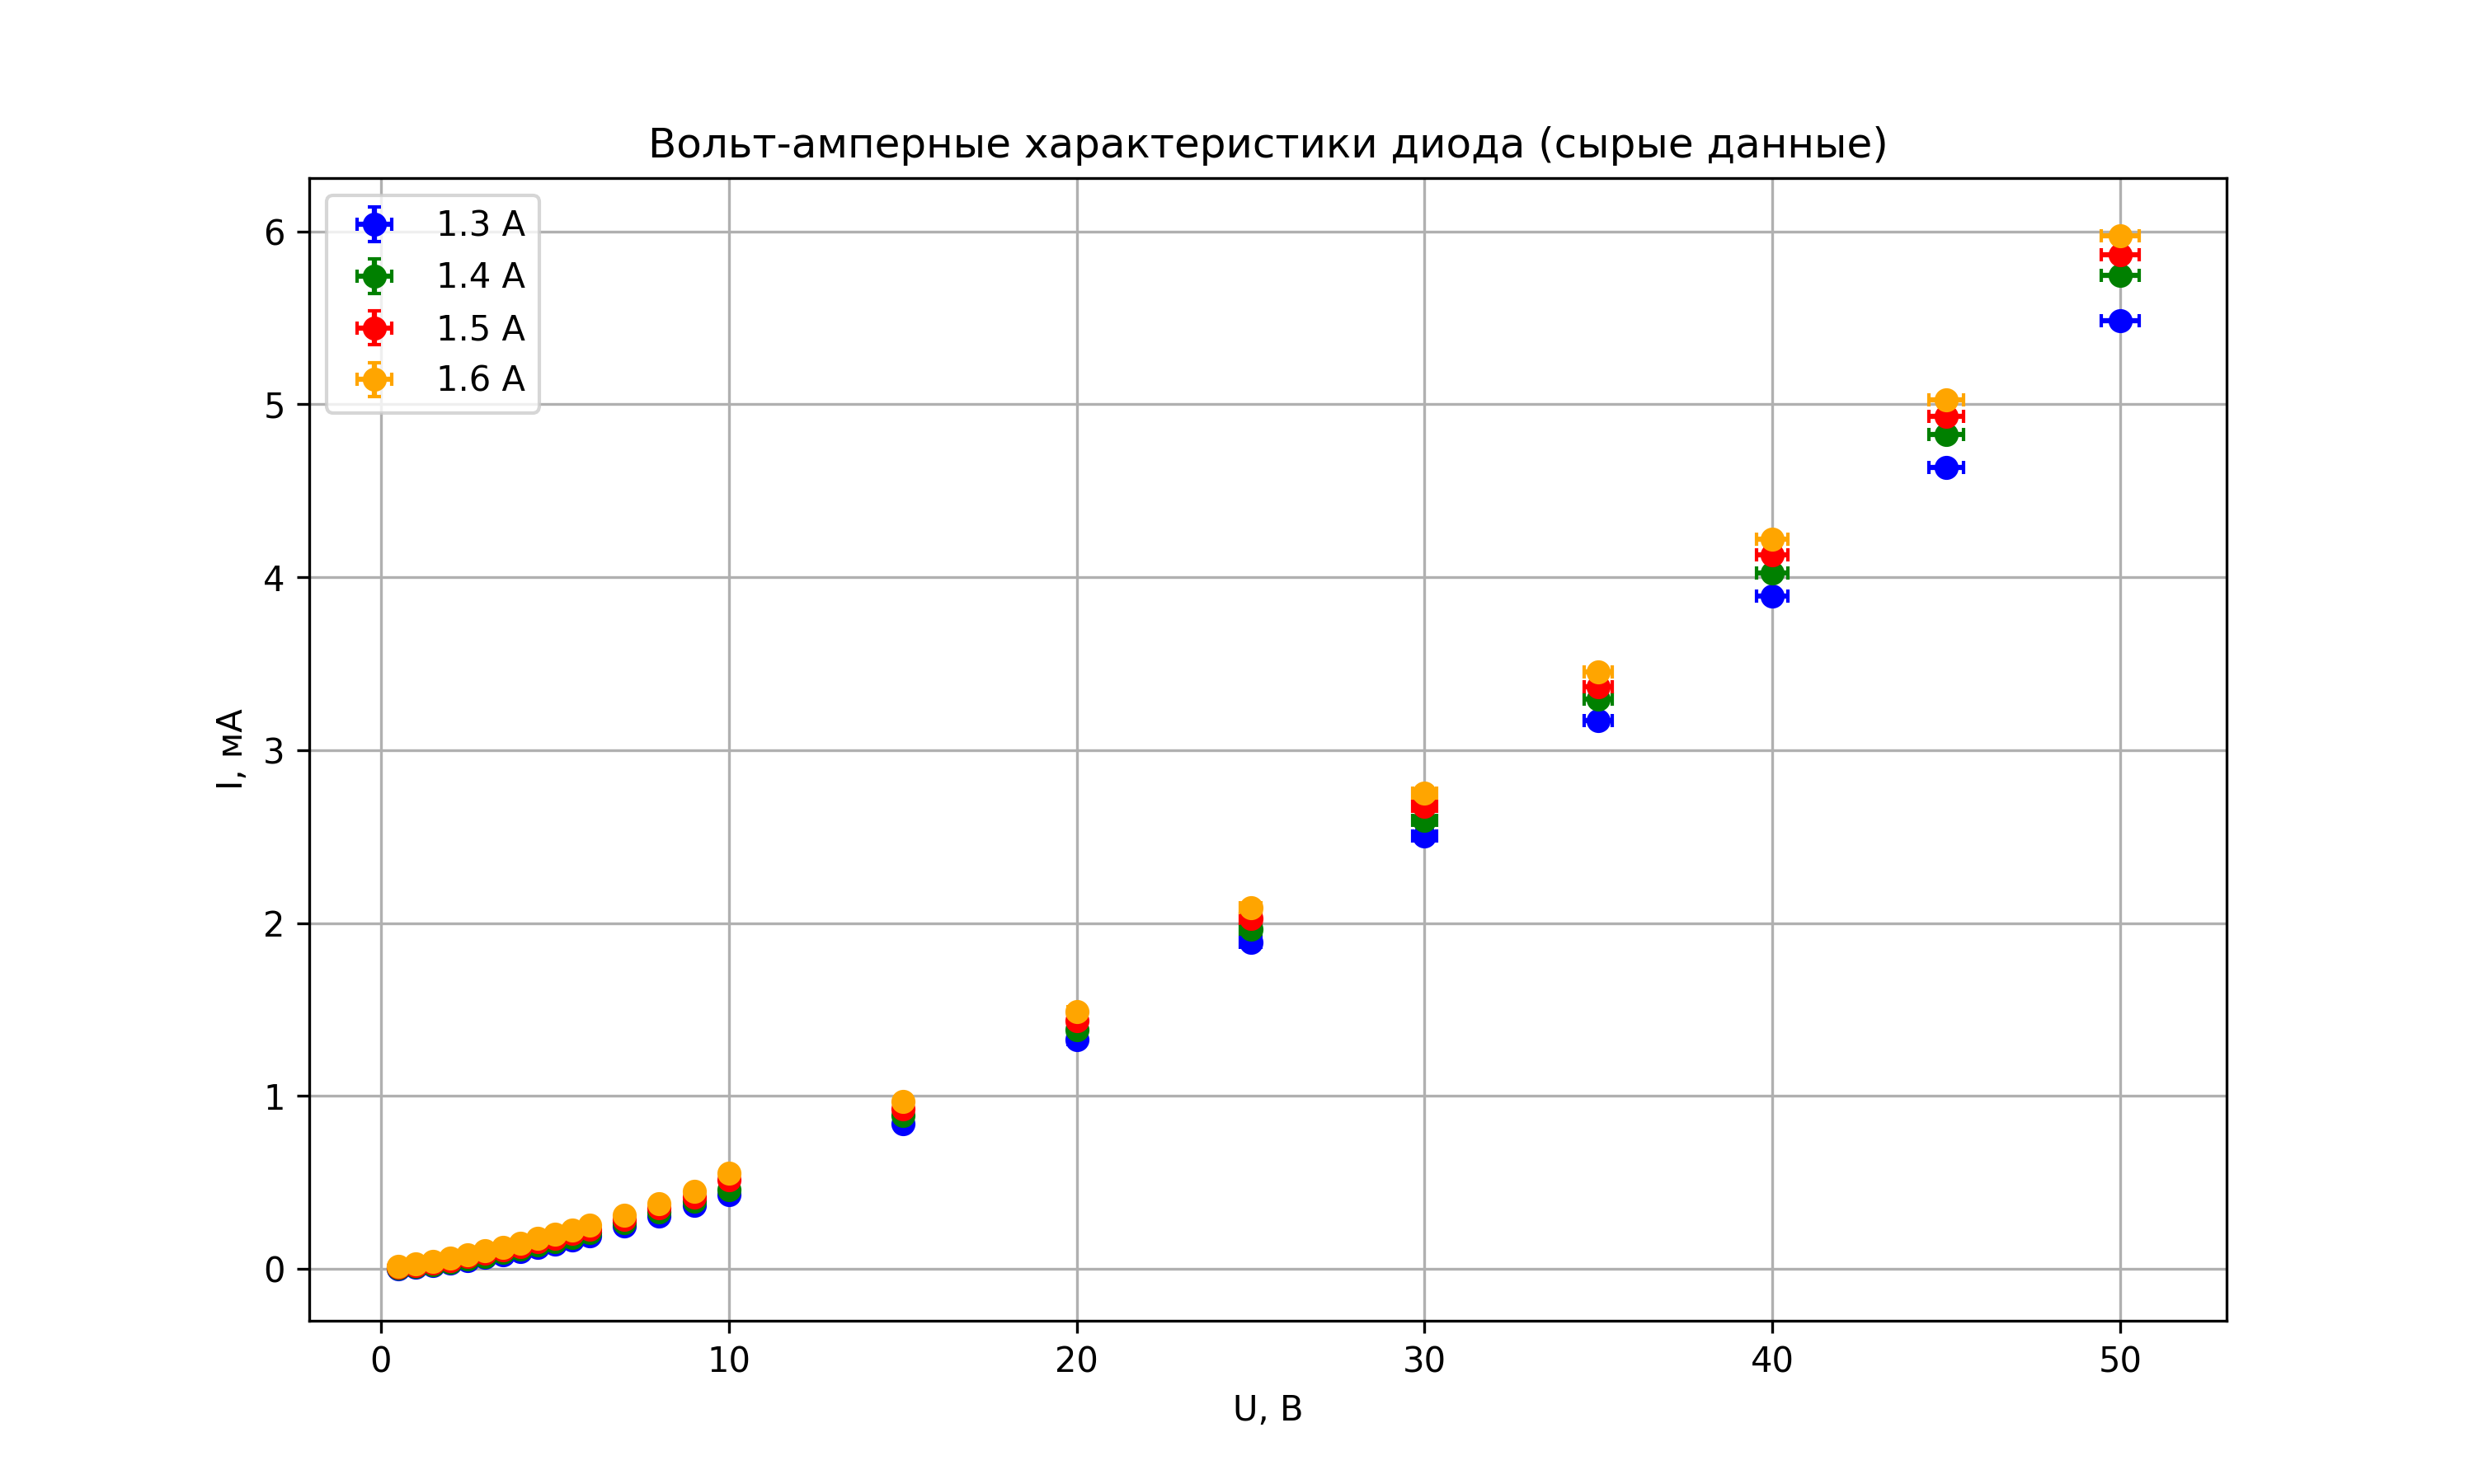
\includegraphics[width=0.8\textwidth]{plots_raw.png}
		\caption{Вольт-амперные характеристики диода (сырые данные)}
		\label{fig:raw}
	\end{figure}
	
	\subsection{Проверка закона «трёх вторых»}
	
	Для проверки закона «трёх вторых» построены графики $I_a$ от $U_a^{3/2}$ (рис.~\ref{fig:plots} и \ref{fig:combined}). В области $U_a \ge 5$ В наблюдается линейная зависимость, проходящая через начало координат. При малых напряжениях ($U < 5$ В) точки отклоняются от прямой, что связано с влиянием начальных скоростей электронов, которыми мы пренебрегли при выводе закона.
	
	\begin{figure}[h]
		\centering
		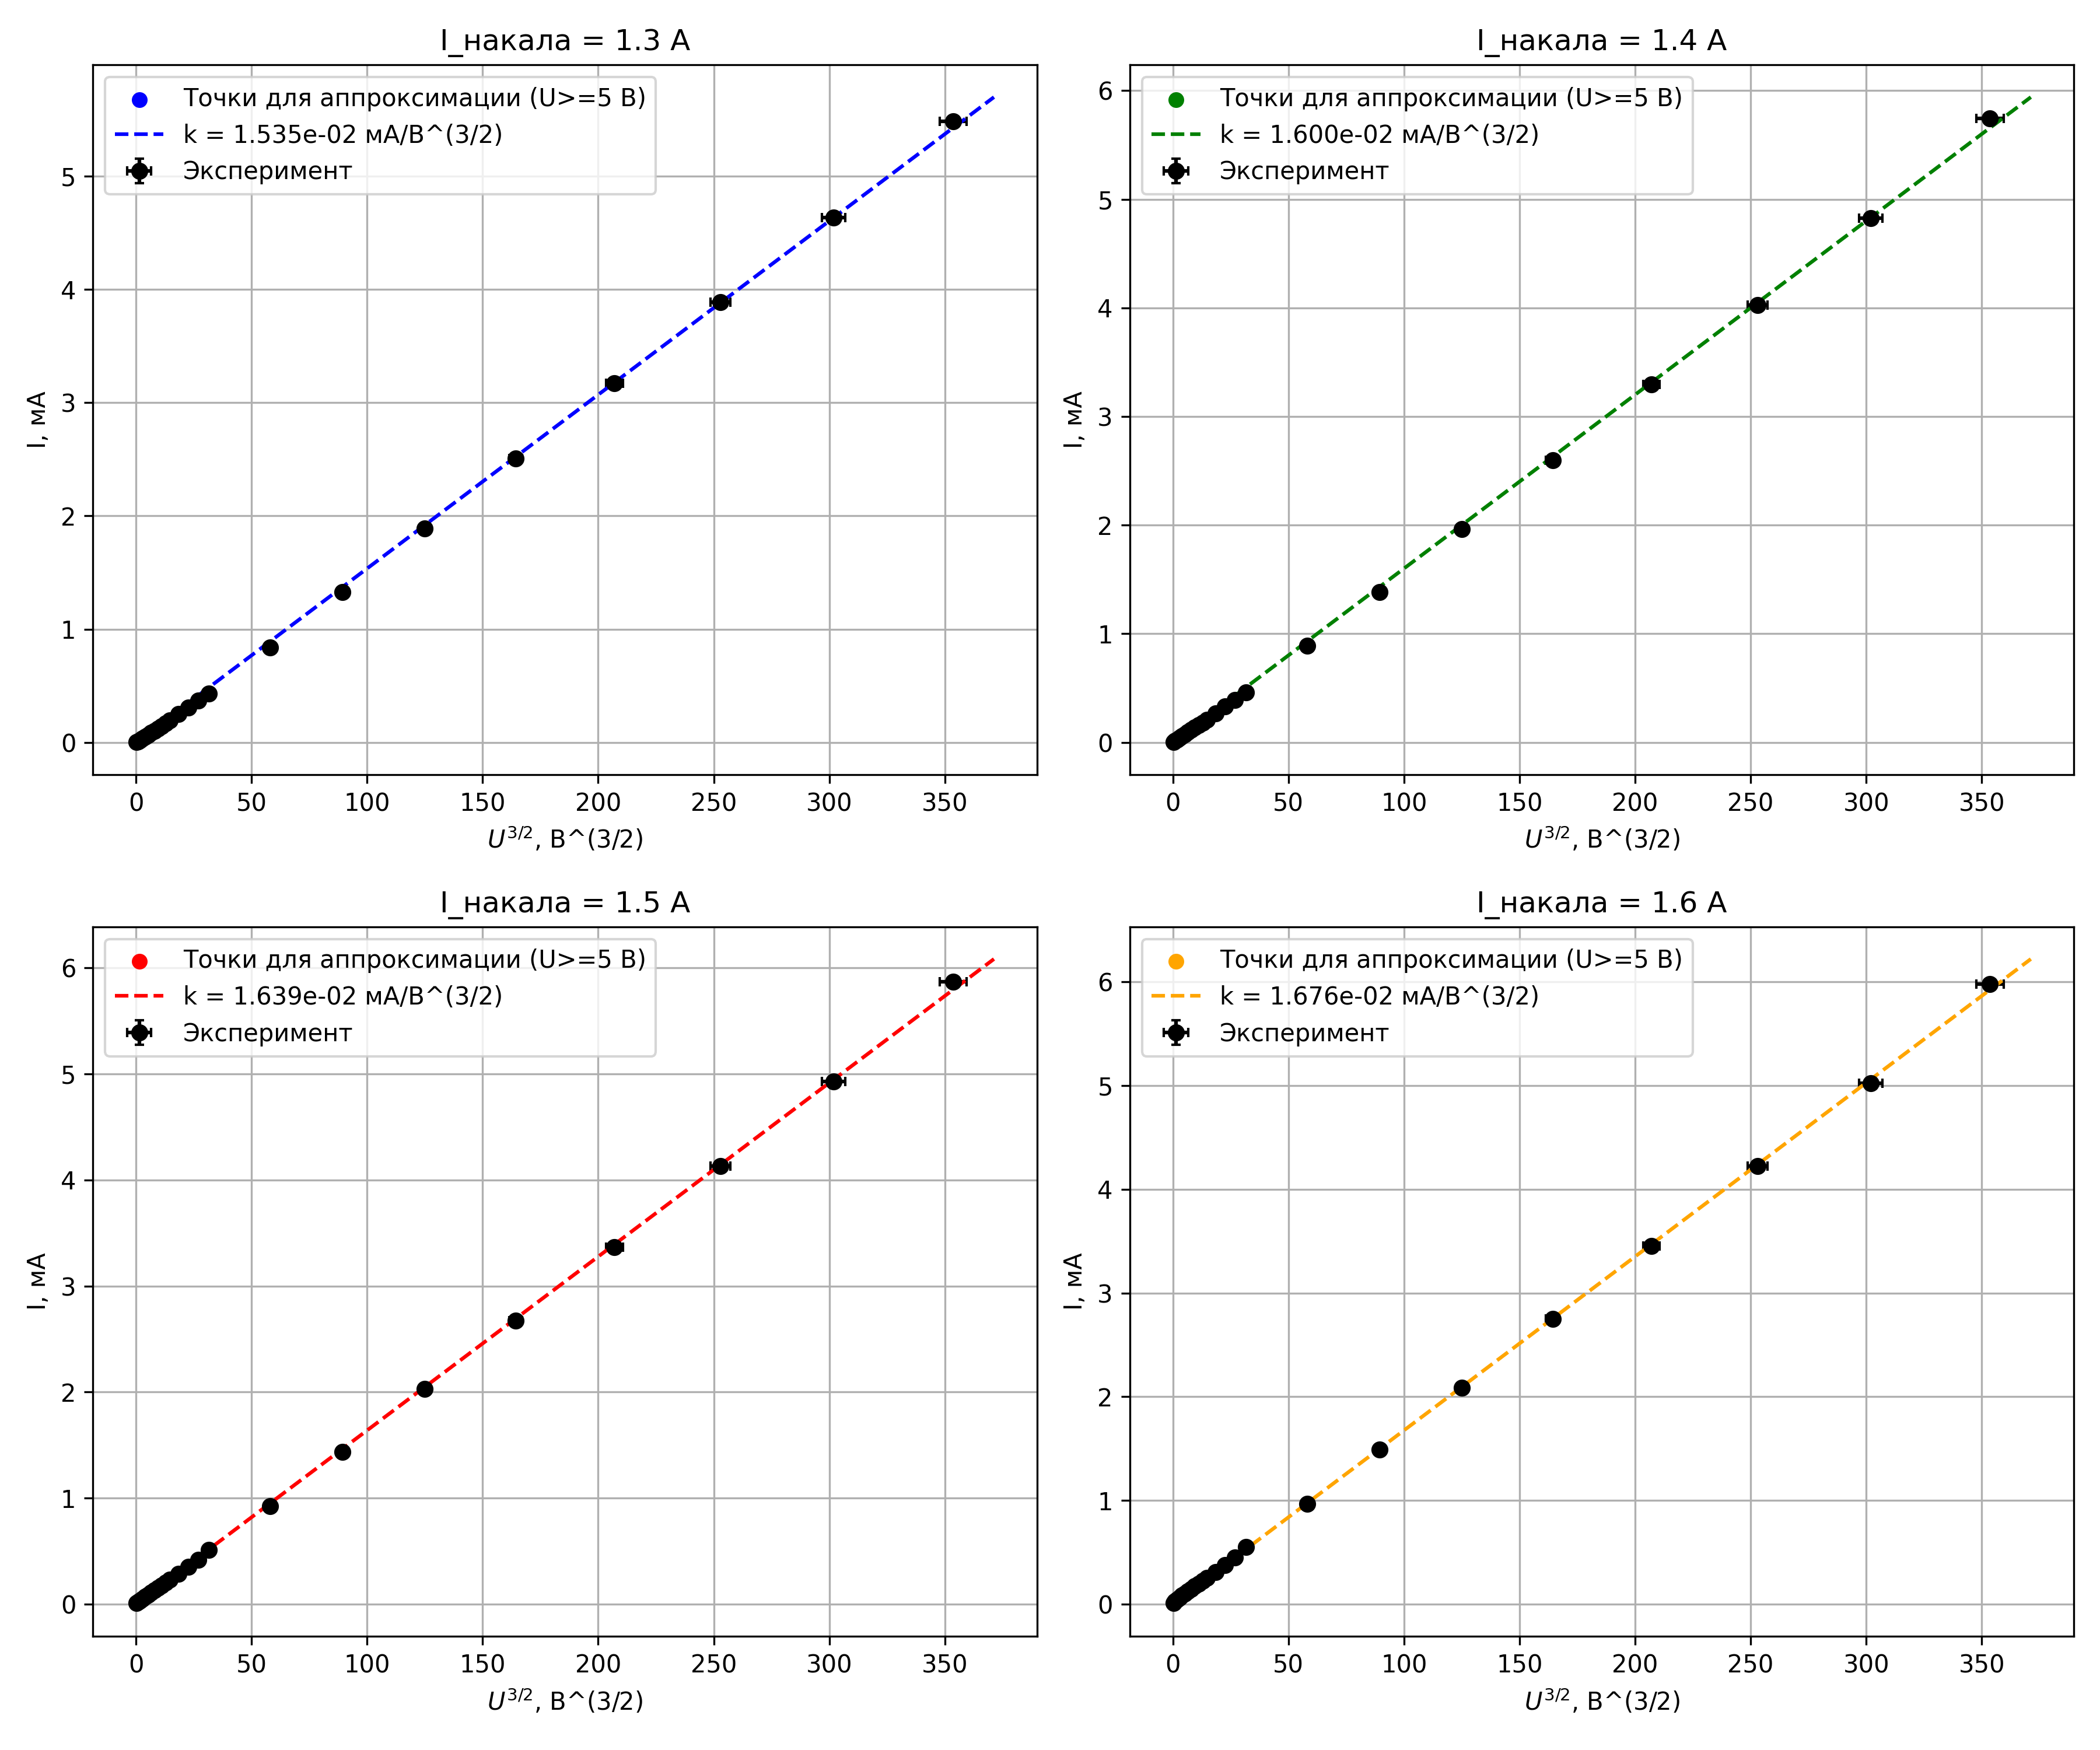
\includegraphics[width=0.9\textwidth]{plots_individual.png}
		\caption{Зависимости $I_a(U_a^{3/2})$ для четырёх токов накала. Аппроксимационные прямые продлены до нуля.}
		\label{fig:plots}
	\end{figure}
	
	\begin{figure}[h]
		\centering
		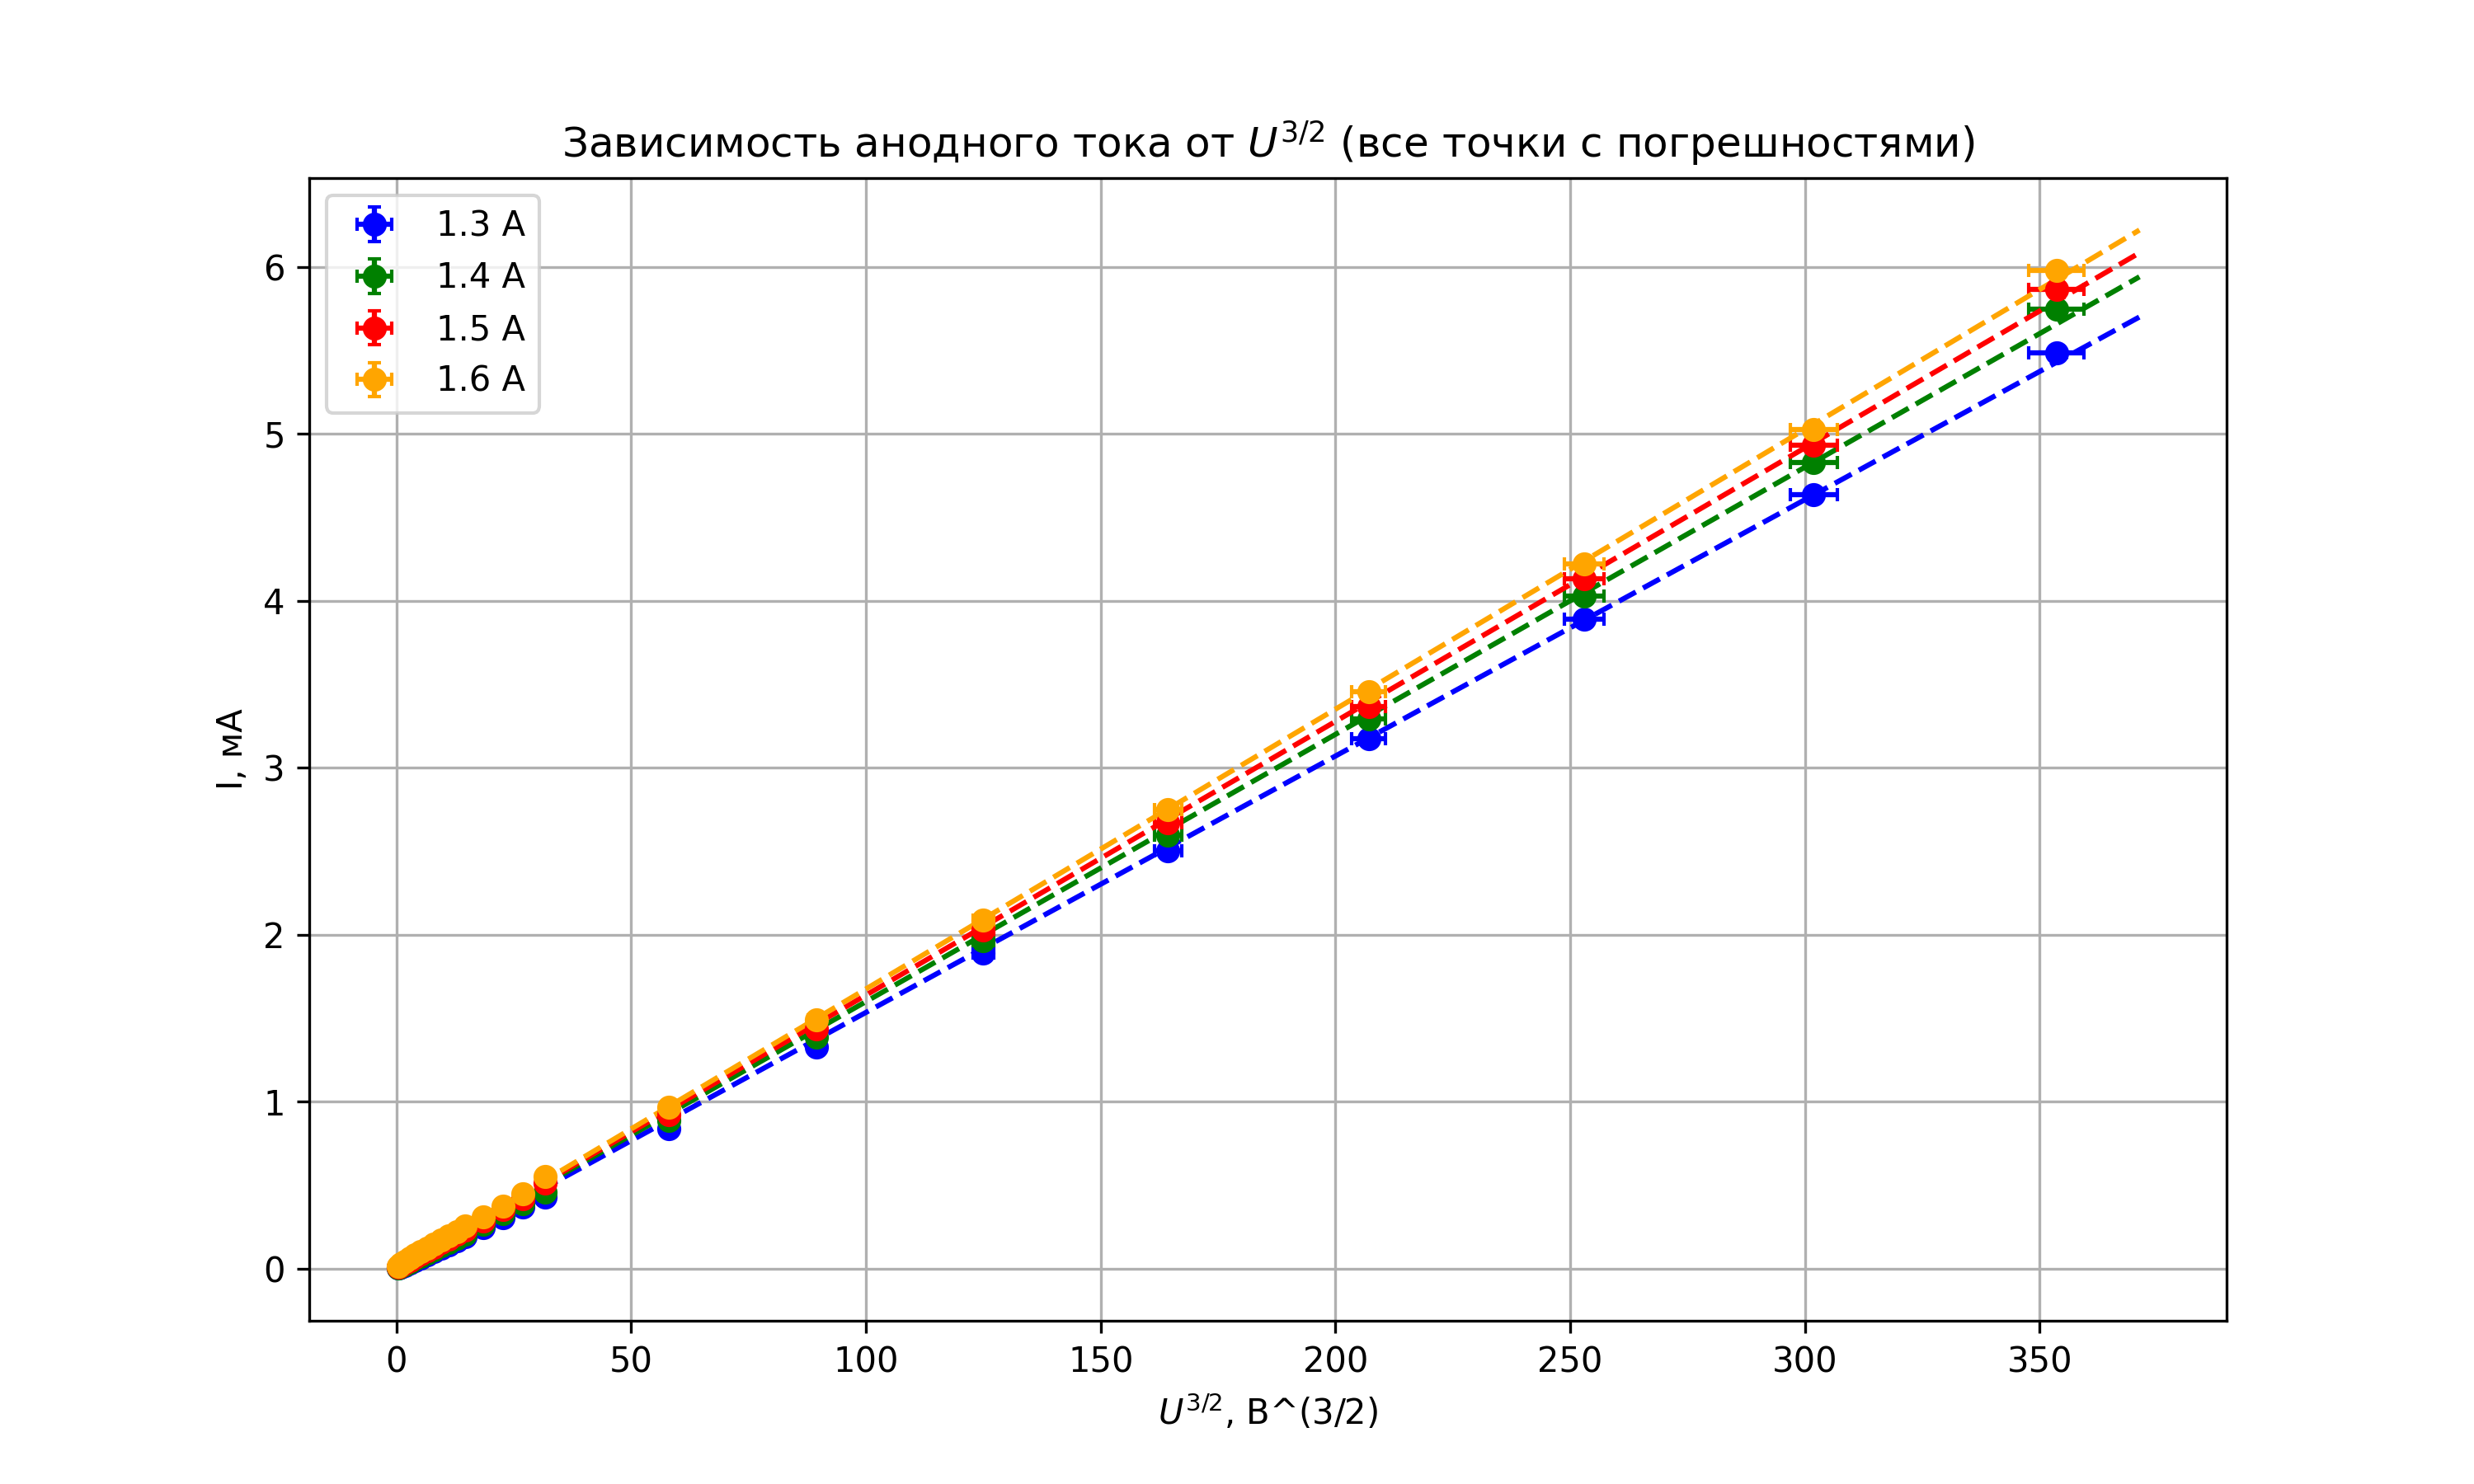
\includegraphics[width=0.9\textwidth]{plots_combined.png}
		\caption{Совмещённые графики с аппроксимациями}
		\label{fig:combined}
	\end{figure}
	
	На рис.~\ref{fig:small} отдельно показана область малых напряжений (0--10 В) для всех четырёх токов накала в координатах $I$ vs $U^{3/2}$. На этом же графике пунктиром изображены теоретические прямые $I = k U^{3/2}$, полученные экстраполяцией линейной области ($U\ge5$ В) для каждой серии. Видно, что при $U < 5$ В (т.е. при малых значениях $U^{3/2}$) экспериментальные точки лежат выше теоретических прямых для всех токов накала. Это объясняется ненулевой начальной скоростью электронов, которая даёт дополнительный вклад в ток при малых напряжениях.
	
	\begin{figure}[h]
		\centering
			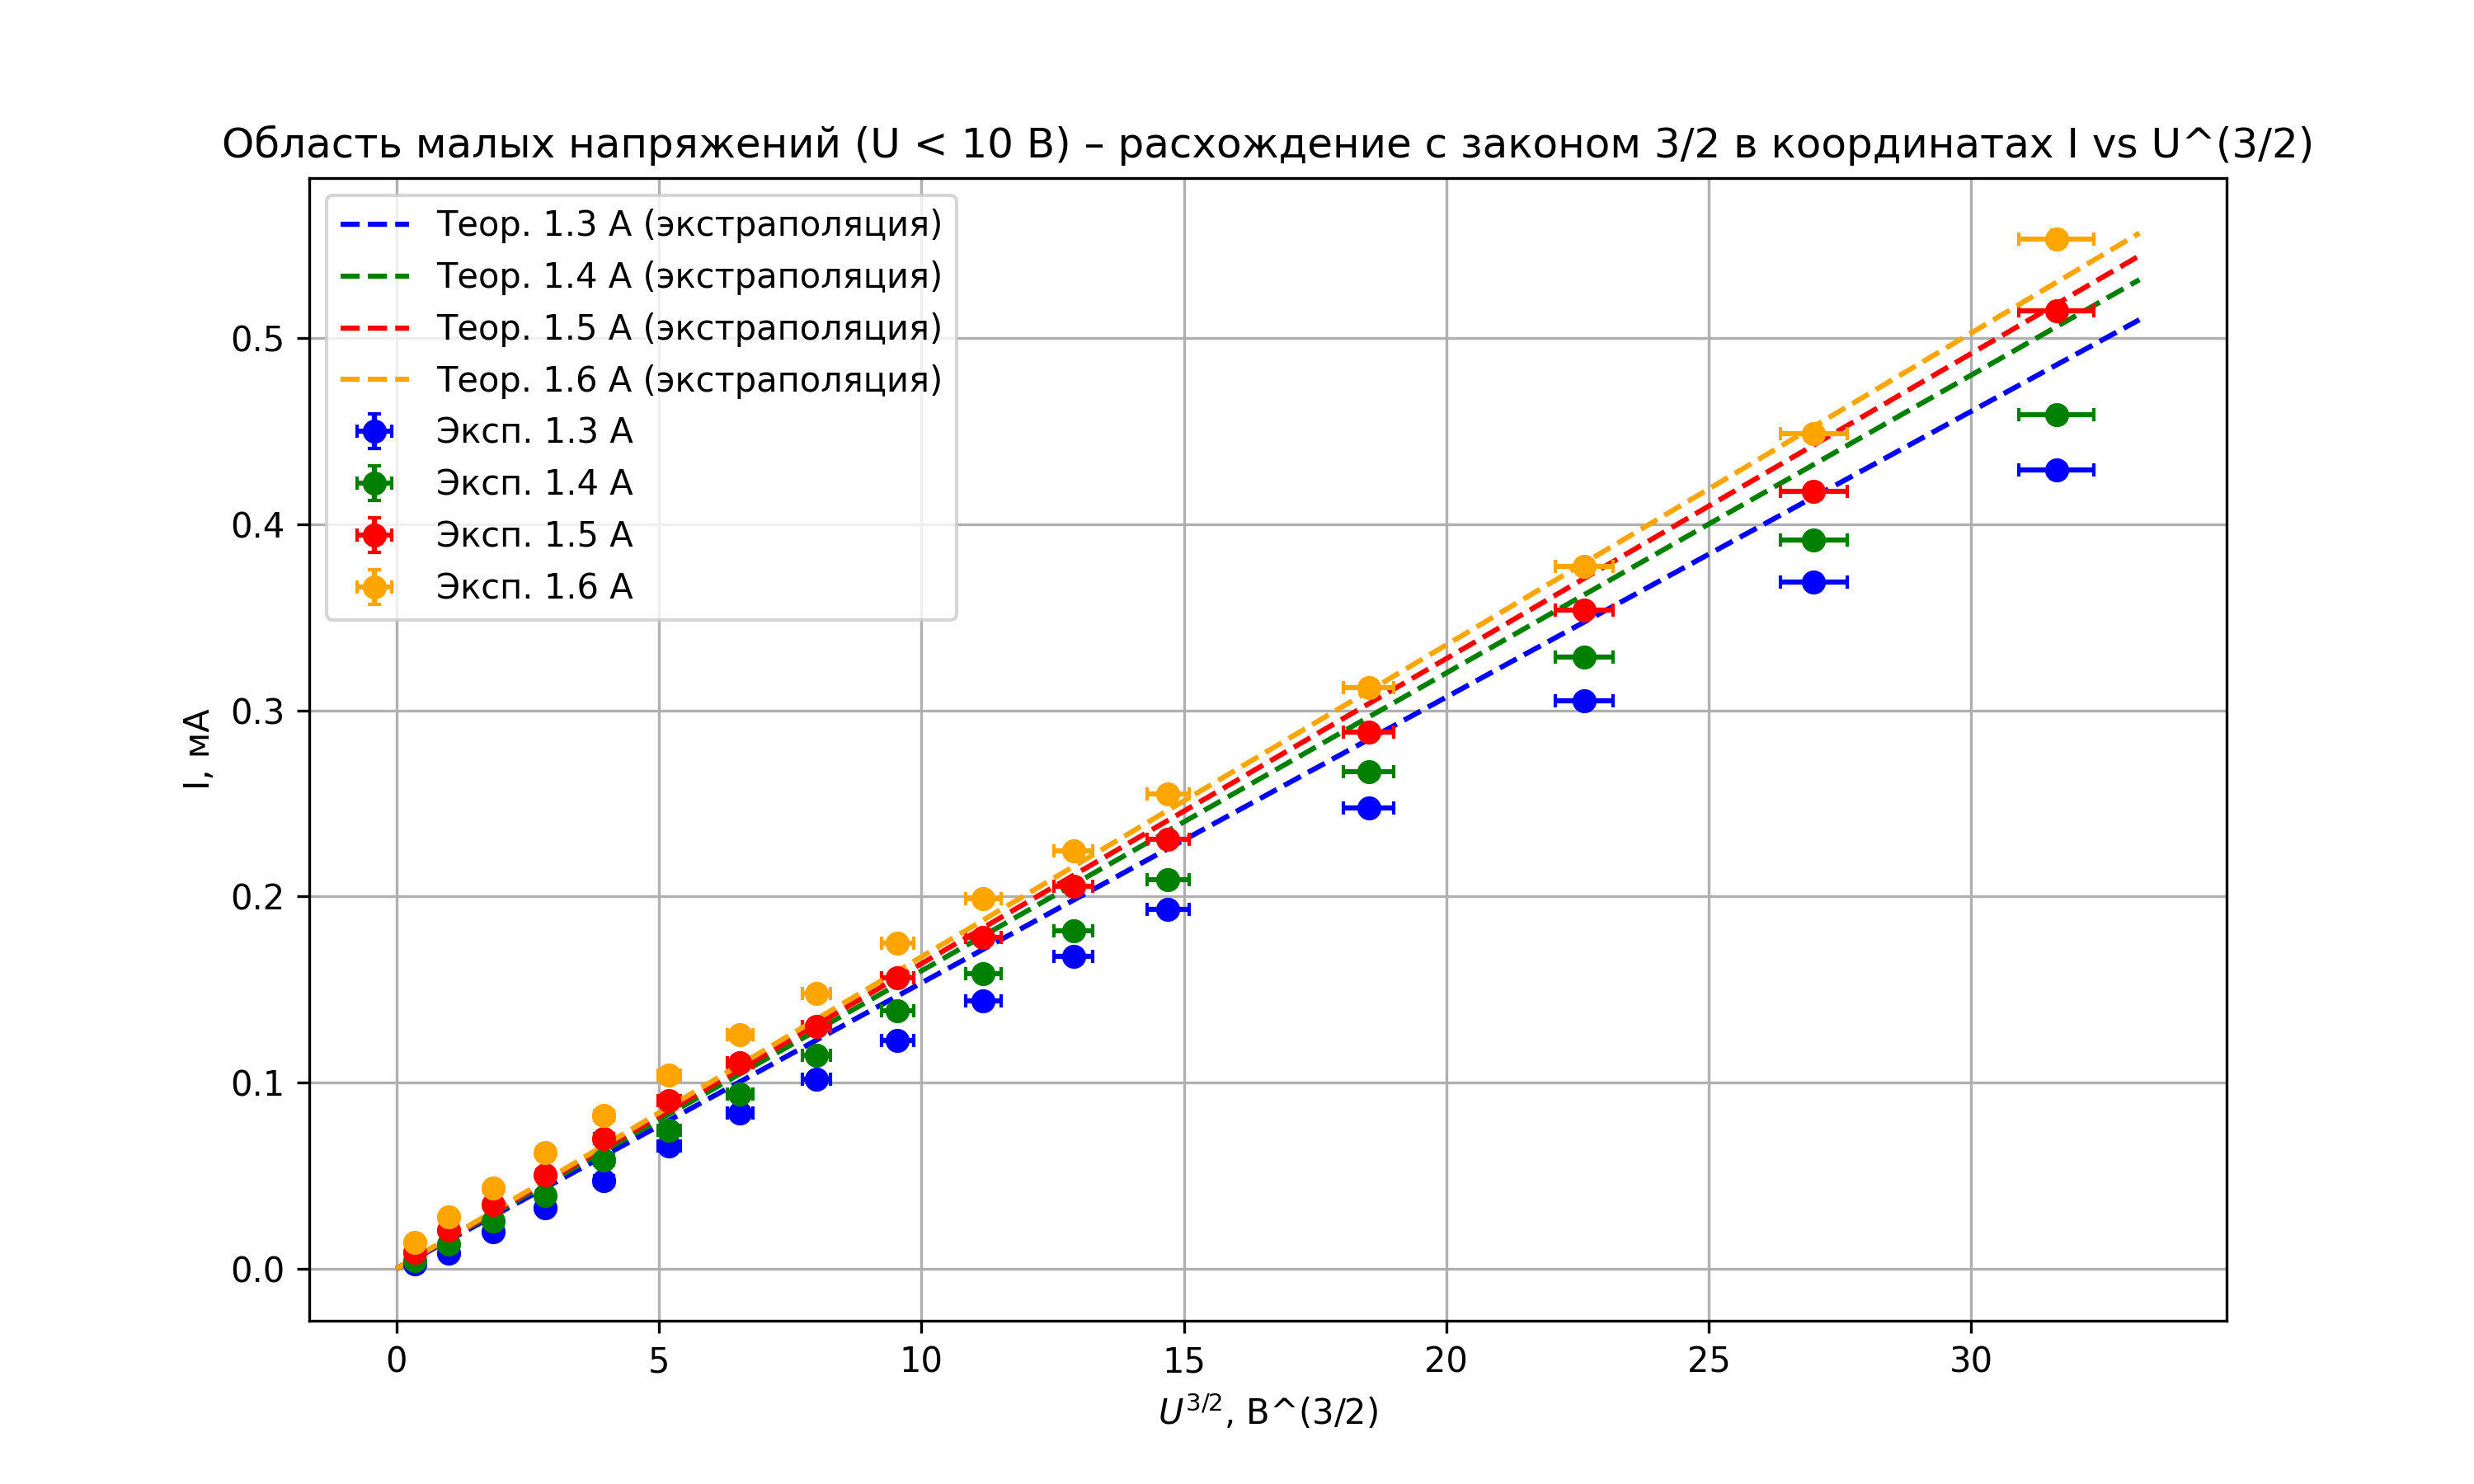
\includegraphics[width=0.9\textwidth]{plots_small.png}
		\caption{Область малых напряжений ($U < 10$ В) -- расхождение с законом 3/2 в координатах $I$ vs $U^{3/2}$. Пунктир -- экстраполяция закона 3/2 из линейной области.}
		\label{fig:small}
	\end{figure}
	
	\subsection{Определение коэффициента наклона}
	
	Аппроксимация прямой $I = k \cdot U^{3/2}$ (без свободного члена) методом наименьших квадратов (с учётом погрешностей) по точкам $U\ge5$ В дала следующие значения коэффициентов $k$ (в мА/В$^{3/2}$):
	
	\begin{table}[h]
		\centering
		\begin{tabular}{|c|c|c|}
			\hline
			Ток накала, А & $k$, мА/В$^{3/2}$ & $\sigma_k$, мА/В$^{3/2}$ \\
			\hline
			1.3 & $1.455 \times 10^{-2}$ & $1.0 \times 10^{-4}$ \\
			1.4 & $1.529 \times 10^{-2}$ & $0.9 \times 10^{-4}$ \\
			1.5 & $1.564 \times 10^{-2}$ & $1.1 \times 10^{-4}$ \\
			1.6 & $1.594 \times 10^{-2}$ & $1.2 \times 10^{-4}$ \\
			\hline
		\end{tabular}
		\caption{Коэффициенты наклона}
		\label{tab:k}
	\end{table}
	
	\subsection{Расчёт удельного заряда электрона}
	
	По формуле
	\[
	\frac{e}{m} = \frac{1}{2} \left( \frac{k \cdot 10^{-3}}{\frac{4}{9} \varepsilon_0 \frac{2\pi l}{r_a} \alpha} \right)^2
	\]
	(здесь $k$ переведён в А/В$^{3/2}$) были вычислены значения $e/m$ для каждого тока накала:
	
	\begin{table}[h]
		\centering
		\begin{tabular}{|c|c|c|}
			\hline
			Ток накала, А & $e/m$, Кл/кг & $\Delta (e/m)$, Кл/кг \\
			\hline
			1.3 & $1.72 \times 10^{11}$ & $0.02 \times 10^{11}$ \\
			1.4 & $1.90 \times 10^{11}$ & $0.02 \times 10^{11}$ \\
			1.5 & $1.99 \times 10^{11}$ & $0.03 \times 10^{11}$ \\
			1.6 & $2.07 \times 10^{11}$ & $0.03 \times 10^{11}$ \\
			\hline
		\end{tabular}
		\caption{Результаты расчёта $e/m$}
		\label{tab:em}
	\end{table}
	
	Среднее значение:
	\[
	\langle e/m \rangle = (1.92 \pm 0.16) \times 10^{11} \text{ Кл/кг}.
	\]
	
	Табличное значение $e/m = 1.758820 \times 10^{11}$ Кл/кг. Полученный результат находится в пределах погрешности эксперимента.
	
	\section{Выводы}
	
	В ходе работы экспериментально подтверждён закон «трёх вторых» для цилиндрического вакуумного диода в области пространственного заряда при достаточно больших напряжениях ($U \ge 5$ В). При малых напряжениях наблюдается отклонение, вызванное начальной тепловой скоростью электронов. Определён удельный заряд электрона:
	\[
	e/m = (1.92 \pm 0.16) \times 10^{11} \text{ Кл/кг},
	\]
	что хорошо согласуется с табличным значением $1.758820 \times 10^{11}$ Кл/кг. Отклонение может быть связано с неточностью определения коэффициента $\alpha$, погрешностью измерений, а также с неучётом начальных скоростей электронов при малых напряжениях.
	
\end{document}